\begin{animateinline}[poster = last, controls]{5}
\multiframe{8}{ra=0+0.25}{
\begin{tikzpicture}[scale=1.5]
\path[use as bounding box] (-3.75,-3.75) rectangle (3.75,3.75);
\draw[->,gray] (-2.5,0) -- (2.5,0) node[right]{$x$};
\draw[->,gray] (0,-2.5) -- (0,2.5) node[above]{$y$};
\draw[blue, thick](0,0)--({\ra},0);
\end{tikzpicture}
}
\newframe
\multiframe{37}{i=1+1}{
\begin{tikzpicture}[scale=1.5]
\path[use as bounding box] (-3.75,-3.75) rectangle (3.75,3.75);
\draw[->,gray] (-2.5,0) -- (2.5,0) node[right]{$x$};
\draw[->,gray] (0,-2.5) -- (0,2.5) node[above]{$y$};
\draw[blue, thick](0,0)--(2,0)node[midway, below]{$r$};
\multido{\r=0+10}{\i}{
\draw[blue, thick]
({2*cos(\r)},{2*sin(\r)})arc(\r:{\r+10}:2);
}
\end{tikzpicture}}
\newframe 
\begin{tikzpicture}[scale=1.5]
\path[use as bounding box] (-3.75,-3.75) rectangle (3.75,3.75);
\draw[->,gray] (-2.5,0) -- (2.5,0) node[right]{$x$};
\draw[->,gray] (0,-2.5) -- (0,2.5) node[above]{$y$};
\draw[blue, thick](0,0)--(2,0)node[midway, below]{$r$};
\draw[blue, thick](2,0)arc(0:360:2);
\draw[red,very thick](2,0)arc(0:180/pi:2)node[midway, right]{\small{1 rad}};
\draw({2*cos(180/pi)},{2*sin(180/pi)})circle(0.02);
\draw[dotted](0,0)--({2*cos(180/pi)},{2*sin(180/pi)});
\draw[fill=pink] (0,0) -- (0.5,0) arc (0:180/pi:0.5);
\filldraw[red]({2*cos(180/pi)},{2*sin(180/pi)})circle(0.04);
\end{tikzpicture}
\newframe
\begin{tikzpicture}[scale=1.5]
\path[use as bounding box] (-3.75,-3.75) rectangle (3.75,3.75);
\draw[->,gray] (-2.5,0) -- (2.5,0) node[right]{$x$};
\draw[->,gray] (0,-2.5) -- (0,2.5) node[above]{$y$};
\draw[blue, thick](0,0)--(2,0)node[midway, below]{$r$};
\draw[blue, thick](2,0)arc(0:360:2);
\draw[red,very thick](2,0)arc(0:180/pi:2)node[midway, right]{\small{1 rad}};
\draw({2*cos(180/pi)},{2*sin(180/pi)})circle(0.02);
\draw[dotted](0,0)--({2*cos(180/pi)},{2*sin(180/pi)});
\draw[fill=pink] (0,0) -- (0.5,0) arc (0:180/pi:0.5);
\filldraw[red]({2*cos(180/pi)},{2*sin(180/pi)})circle(0.04);
\begin{scope}[rotate around={180/pi:(0,0)}]
\draw[red,very thick](2,0)arc(0:180/pi:2);
\draw({2*cos(180/pi)},{2*sin(180/pi)})circle(0.02);
\draw[dotted](0,0)--({2*cos(180/pi)},{2*sin(180/pi)});
\draw[fill=pink] (0,0) -- (0.5,0) arc (0:180/pi:0.5);
\filldraw[red]({2*cos(180/pi)},{2*sin(180/pi)})circle(0.04);
\end{scope}
\end{tikzpicture}
\newframe
\begin{tikzpicture}[scale=1.5]
\path[use as bounding box] (-3.75,-3.75) rectangle (3.75,3.75);
\draw[->,gray] (-2.5,0) -- (2.5,0) node[right]{$x$};
\draw[->,gray] (0,-2.5) -- (0,2.5) node[above]{$y$};
\draw[blue, thick](0,0)--(2,0)node[midway, below]{$r$};
\draw[blue, thick](2,0)arc(0:360:2);
\draw[red,very thick](2,0)arc(0:180/pi:2)node[midway, right]{\small{1 rad}};
\draw({2*cos(180/pi)},{2*sin(180/pi)})circle(0.02);
\draw(0,0)--({2*cos(180/pi)},{2*sin(180/pi)});
\draw[fill=pink] (0,0) -- (0.5,0) arc (0:180/pi:0.5);
\filldraw[red]({2*cos(180/pi)},{2*sin(180/pi)})circle(0.04);
\begin{scope}[rotate around={180/pi:(0,0)}]
\draw[red,very thick](2,0)arc(0:180/pi:2);
\draw({2*cos(180/pi)},{2*sin(180/pi)})circle(0.02);
\draw[dotted](0,0)--({2*cos(180/pi)},{2*sin(180/pi)});
\draw[fill=pink] (0,0) -- (0.5,0) arc (0:180/pi:0.5);
\filldraw[red]({2*cos(180/pi)},{2*sin(180/pi)})circle(0.04);
\end{scope}
\begin{scope}[rotate around={360/pi:(0,0)}]
\draw[red,very thick](2,0)arc(0:180/pi:2);
\draw({2*cos(180/pi)},{2*sin(180/pi)})circle(0.02);
\draw[dotted](0,0)--({2*cos(180/pi)},{2*sin(180/pi)});
\draw[fill=pink] (0,0) -- (0.5,0) arc (0:180/pi:0.5);
\filldraw[red]({2*cos(180/pi)},{2*sin(180/pi)})circle(0.04);
\end{scope}
\end{tikzpicture}
\newframe
\begin{tikzpicture}[scale=1.5]
\path[use as bounding box] (-3.75,-3.75) rectangle (3.75,3.75);
\draw[->,gray] (-2.5,0) -- (2.5,0) node[right]{$x$};
\draw[->,gray] (0,-2.5) -- (0,2.5) node[above]{$y$};
\draw[blue, thick](0,0)--(2,0)node[midway, below]{$r$};
\draw[blue, thick](2,0)arc(0:360:2);
\draw[red,very thick](2,0)arc(0:180/pi:2)node[midway, right]{\small{1 rad}};
\draw({2*cos(180/pi)},{2*sin(180/pi)})circle(0.02);
\draw(0,0)--({2*cos(180/pi)},{2*sin(180/pi)});
\draw[fill=pink] (0,0) -- (0.5,0) arc (0:180/pi:0.5);
\filldraw[red]({2*cos(180/pi)},{2*sin(180/pi)})circle(0.04);
\begin{scope}[rotate around={180/pi:(0,0)}]
\draw[red,very thick](2,0)arc(0:180/pi:2);
\draw({2*cos(180/pi)},{2*sin(180/pi)})circle(0.02);
\draw[dotted](0,0)--({2*cos(180/pi)},{2*sin(180/pi)});
\draw[fill=pink] (0,0) -- (0.5,0) arc (0:180/pi:0.5);
\filldraw[red]({2*cos(180/pi)},{2*sin(180/pi)})circle(0.04);
\end{scope}
\begin{scope}[rotate around={360/pi:(0,0)}]
\draw[red,very thick](2,0)arc(0:180/pi:2);
\draw({2*cos(180/pi)},{2*sin(180/pi)})circle(0.02);
\draw[dotted](0,0)--({2*cos(180/pi)},{2*sin(180/pi)});
\draw[fill=pink] (0,0) -- (0.5,0) arc (0:180/pi:0.5);
\filldraw[red]({2*cos(180/pi)},{2*sin(180/pi)})circle(0.04);
\end{scope}
\end{tikzpicture}
\newframe
\begin{tikzpicture}[scale=1.5]
\path[use as bounding box] (-3.75,-3.75) rectangle (3.75,3.75);
\draw[->,gray] (-2.5,0) -- (2.5,0) node[right]{$x$};
\draw[->,gray] (0,-2.5) -- (0,2.5) node[above]{$y$};
\draw[blue, thick](0,0)--(2,0)node[midway, below]{$r$};
\draw[blue, thick](2,0)arc(0:360:2);
\draw[red,very thick](2,0)arc(0:180/pi:2)node[midway, right]{\small{1 rad}};
\draw({2*cos(180/pi)},{2*sin(180/pi)})circle(0.02);
\draw(0,0)--({2*cos(180/pi)},{2*sin(180/pi)});
\draw[fill=pink] (0,0) -- (0.5,0) arc (0:180/pi:0.5);
\filldraw[red]({2*cos(180/pi)},{2*sin(180/pi)})circle(0.04);
\begin{scope}[rotate around={180/pi:(0,0)}]
\draw[red,very thick](2,0)arc(0:180/pi:2);
\draw({2*cos(180/pi)},{2*sin(180/pi)})circle(0.02);
\draw[dotted](0,0)--({2*cos(180/pi)},{2*sin(180/pi)});
\draw[fill=pink] (0,0) -- (0.5,0) arc (0:180/pi:0.5);
\filldraw[red]({2*cos(180/pi)},{2*sin(180/pi)})circle(0.04);
\end{scope}
\begin{scope}[rotate around={360/pi:(0,0)}]
\draw[red,very thick](2,0)arc(0:180/pi:2);
\draw({2*cos(180/pi)},{2*sin(180/pi)})circle(0.02);
\draw[dotted](0,0)--({2*cos(180/pi)},{2*sin(180/pi)});
\draw[fill=pink] (0,0) -- (0.5,0) arc (0:180/pi:0.5);
\filldraw[red]({2*cos(180/pi)},{2*sin(180/pi)})circle(0.04);
\end{scope}
\begin{scope}[rotate around={540/pi:(0,0)}]
\draw[red,very thick](2,0)arc(0:180/pi:2);
\draw({2*cos(180/pi)},{2*sin(180/pi)})circle(0.02);
\draw[dotted](0,0)--({2*cos(180/pi)},{2*sin(180/pi)});
\draw[fill=pink] (0,0) -- (0.5,0) arc (0:180/pi:0.5);
\filldraw[red]({2*cos(180/pi)},{2*sin(180/pi)})circle(0.04);
\end{scope}
\end{tikzpicture}
\newframe
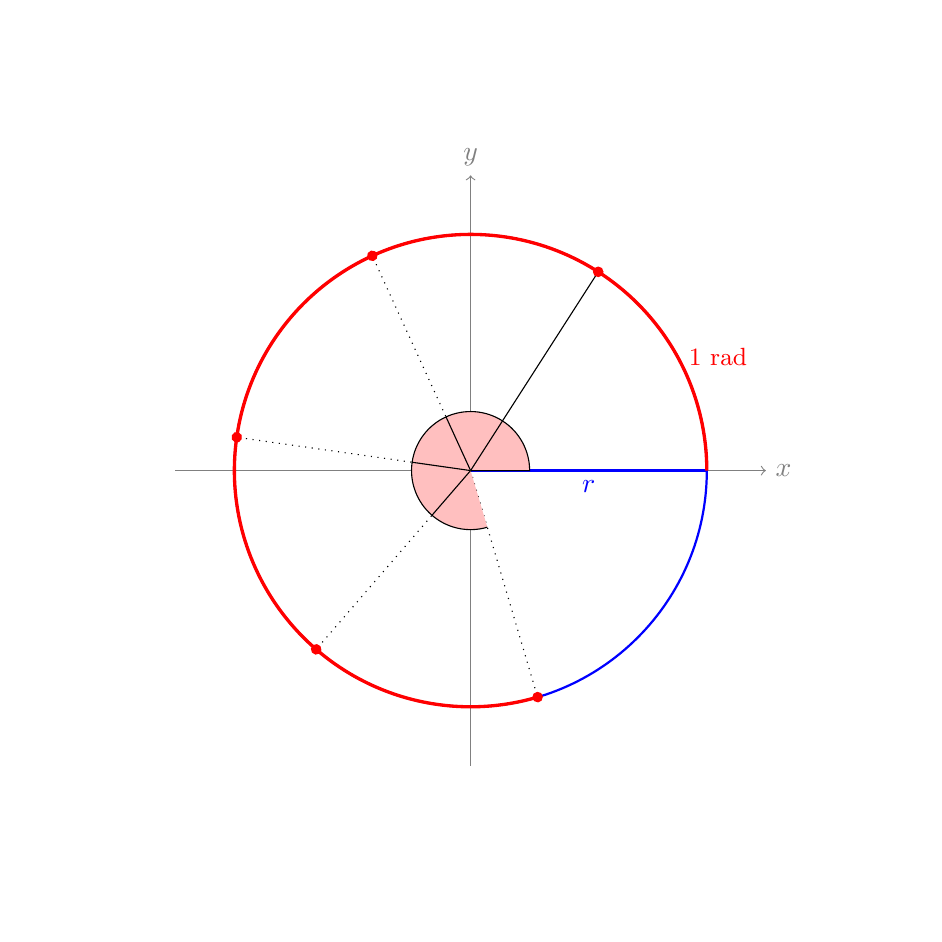
\begin{tikzpicture}[scale=1.5]
\path[use as bounding box] (-3.75,-3.75) rectangle (3.75,3.75);
\draw[->,gray] (-2.5,0) -- (2.5,0) node[right]{$x$};
\draw[->,gray] (0,-2.5) -- (0,2.5) node[above]{$y$};
\draw[blue, thick](0,0)--(2,0)node[midway, below]{$r$};
\draw[blue, thick](2,0)arc(0:360:2);
\draw[red,very thick](2,0)arc(0:180/pi:2)node[midway, right]{\small{1 rad}};
\draw({2*cos(180/pi)},{2*sin(180/pi)})circle(0.02);
\draw(0,0)--({2*cos(180/pi)},{2*sin(180/pi)});
\draw[fill=pink] (0,0) -- (0.5,0) arc (0:180/pi:0.5);
\filldraw[red]({2*cos(180/pi)},{2*sin(180/pi)})circle(0.04);
\begin{scope}[rotate around={180/pi:(0,0)}]
\draw[red,very thick](2,0)arc(0:180/pi:2);
\draw({2*cos(180/pi)},{2*sin(180/pi)})circle(0.02);
\draw[dotted](0,0)--({2*cos(180/pi)},{2*sin(180/pi)});
\draw[fill=pink] (0,0) -- (0.5,0) arc (0:180/pi:0.5);
\filldraw[red]({2*cos(180/pi)},{2*sin(180/pi)})circle(0.04);
\end{scope}
\begin{scope}[rotate around={360/pi:(0,0)}]
\draw[red,very thick](2,0)arc(0:180/pi:2);
\draw({2*cos(180/pi)},{2*sin(180/pi)})circle(0.02);
\draw[dotted](0,0)--({2*cos(180/pi)},{2*sin(180/pi)});
\draw[fill=pink] (0,0) -- (0.5,0) arc (0:180/pi:0.5);
\filldraw[red]({2*cos(180/pi)},{2*sin(180/pi)})circle(0.04);
\end{scope}
\begin{scope}[rotate around={540/pi:(0,0)}]
\draw[red,very thick](2,0)arc(0:180/pi:2);
\draw({2*cos(180/pi)},{2*sin(180/pi)})circle(0.02);
\draw[dotted](0,0)--({2*cos(180/pi)},{2*sin(180/pi)});
\draw[fill=pink] (0,0) -- (0.5,0) arc (0:180/pi:0.5);
\filldraw[red]({2*cos(180/pi)},{2*sin(180/pi)})circle(0.04);
\end{scope}
\begin{scope}[rotate around={720/pi:(0,0)}]
\draw[red,very thick](2,0)arc(0:180/pi:2);
\draw({2*cos(180/pi)},{2*sin(180/pi)})circle(0.02);
\draw[dotted](0,0)--({2*cos(180/pi)},{2*sin(180/pi)});
\draw[fill=pink] (0,0) -- (0.5,0) arc (0:180/pi:0.5);
\filldraw[red]({2*cos(180/pi)},{2*sin(180/pi)})circle(0.04);
\end{scope}
\end{tikzpicture}
\newframe
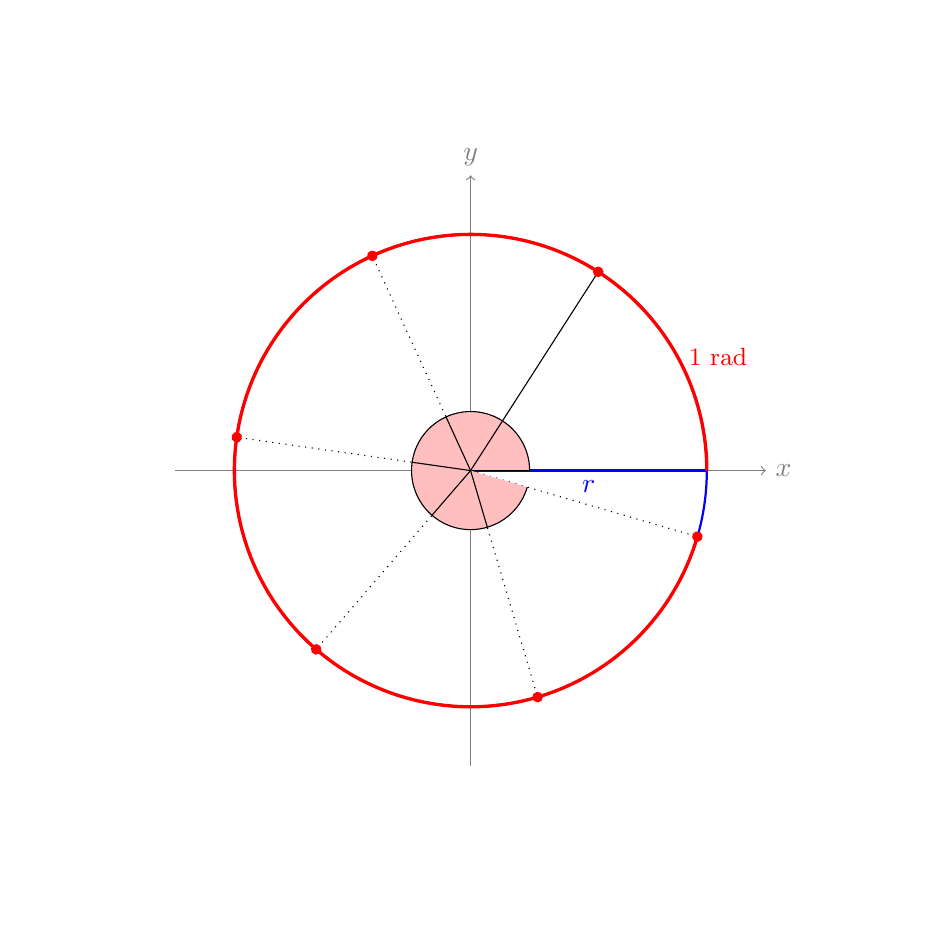
\begin{tikzpicture}[scale=1.5]
\path[use as bounding box] (-3.75,-3.75) rectangle (3.75,3.75);
\draw[->,gray] (-2.5,0) -- (2.5,0) node[right]{$x$};
\draw[->,gray] (0,-2.5) -- (0,2.5) node[above]{$y$};
\draw[blue, thick](0,0)--(2,0)node[midway, below]{$r$};
\draw[blue, thick](2,0)arc(0:360:2);
\draw[red,very thick](2,0)arc(0:180/pi:2)node[midway, right]{\small{1 rad}};
\draw({2*cos(180/pi)},{2*sin(180/pi)})circle(0.02);
\draw(0,0)--({2*cos(180/pi)},{2*sin(180/pi)});
\draw[fill=pink] (0,0) -- (0.5,0) arc (0:180/pi:0.5);
\filldraw[red]({2*cos(180/pi)},{2*sin(180/pi)})circle(0.04);
\begin{scope}[rotate around={180/pi:(0,0)}]
\draw[red,very thick](2,0)arc(0:180/pi:2);
\draw({2*cos(180/pi)},{2*sin(180/pi)})circle(0.02);
\draw[dotted](0,0)--({2*cos(180/pi)},{2*sin(180/pi)});
\draw[fill=pink] (0,0) -- (0.5,0) arc (0:180/pi:0.5);
\filldraw[red]({2*cos(180/pi)},{2*sin(180/pi)})circle(0.04);
\end{scope}
\begin{scope}[rotate around={360/pi:(0,0)}]
\draw[red,very thick](2,0)arc(0:180/pi:2);
\draw({2*cos(180/pi)},{2*sin(180/pi)})circle(0.02);
\draw[dotted](0,0)--({2*cos(180/pi)},{2*sin(180/pi)});
\draw[fill=pink] (0,0) -- (0.5,0) arc (0:180/pi:0.5);
\filldraw[red]({2*cos(180/pi)},{2*sin(180/pi)})circle(0.04);
\end{scope}
\begin{scope}[rotate around={540/pi:(0,0)}]
\draw[red,very thick](2,0)arc(0:180/pi:2);
\draw({2*cos(180/pi)},{2*sin(180/pi)})circle(0.02);
\draw[dotted](0,0)--({2*cos(180/pi)},{2*sin(180/pi)});
\draw[fill=pink] (0,0) -- (0.5,0) arc (0:180/pi:0.5);
\filldraw[red]({2*cos(180/pi)},{2*sin(180/pi)})circle(0.04);
\end{scope}
\begin{scope}[rotate around={720/pi:(0,0)}]
\draw[red,very thick](2,0)arc(0:180/pi:2);
\draw({2*cos(180/pi)},{2*sin(180/pi)})circle(0.02);
\draw[dotted](0,0)--({2*cos(180/pi)},{2*sin(180/pi)});
\draw[fill=pink] (0,0) -- (0.5,0) arc (0:180/pi:0.5);
\filldraw[red]({2*cos(180/pi)},{2*sin(180/pi)})circle(0.04);
\end{scope}
\begin{scope}[rotate around={900/pi:(0,0)}]
\draw[red,very thick](2,0)arc(0:180/pi:2);
\draw({2*cos(180/pi)},{2*sin(180/pi)})circle(0.02);
\draw[dotted](0,0)--({2*cos(180/pi)},{2*sin(180/pi)});
\draw[fill=pink] (0,0) -- (0.5,0) arc (0:180/pi:0.5);
\filldraw[red]({2*cos(180/pi)},{2*sin(180/pi)})circle(0.04);
\end{scope}
\end{tikzpicture}
\newframe
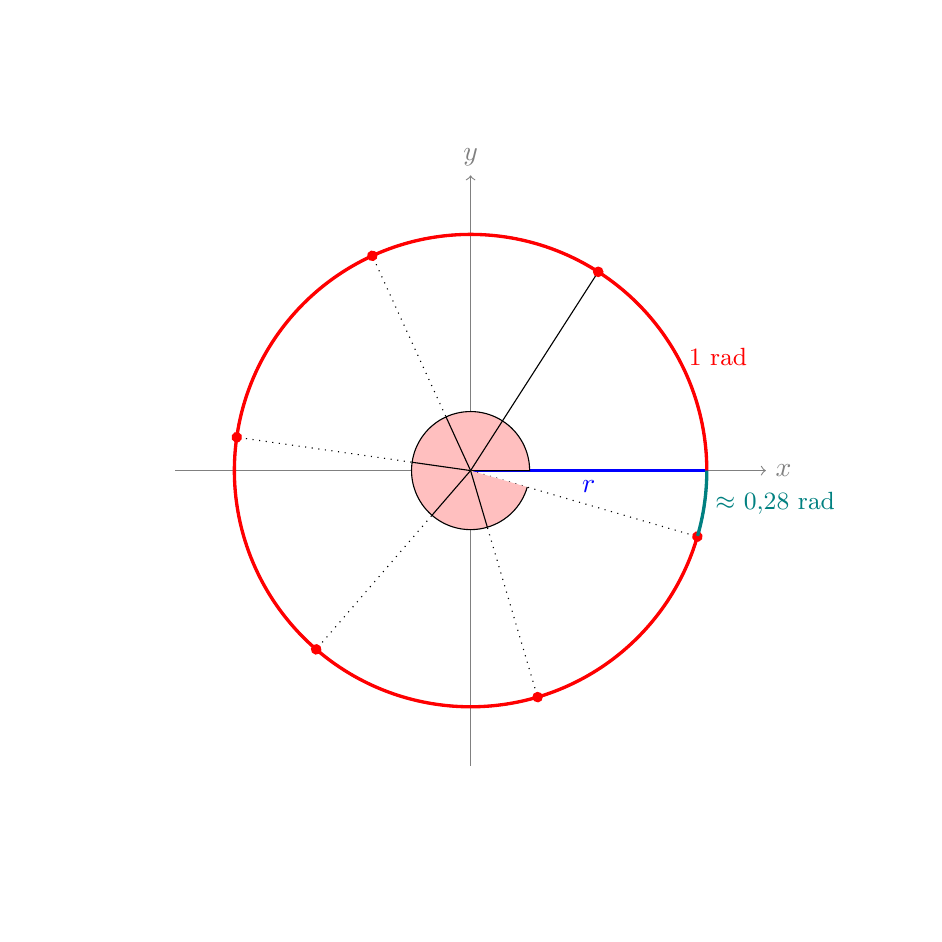
\begin{tikzpicture}[scale=1.5]
\path[use as bounding box] (-3.75,-3.75) rectangle (3.75,3.75);
\draw[->,gray] (-2.5,0) -- (2.5,0) node[right]{$x$};
\draw[->,gray] (0,-2.5) -- (0,2.5) node[above]{$y$};
\draw[blue, thick](0,0)--(2,0)node[midway, below]{$r$};
\draw[blue, thick](2,0)arc(0:360:2);
\draw[red,very thick](2,0)arc(0:180/pi:2)node[midway, right]{\small{1 rad}};
\draw({2*cos(180/pi)},{2*sin(180/pi)})circle(0.02);
\draw(0,0)--({2*cos(180/pi)},{2*sin(180/pi)});
\draw[fill=pink] (0,0) -- (0.5,0) arc (0:180/pi:0.5);
\filldraw[red]({2*cos(180/pi)},{2*sin(180/pi)})circle(0.04);
\begin{scope}[rotate around={180/pi:(0,0)}]
\draw[red,very thick](2,0)arc(0:180/pi:2);
\draw({2*cos(180/pi)},{2*sin(180/pi)})circle(0.02);
\draw[dotted](0,0)--({2*cos(180/pi)},{2*sin(180/pi)});
\draw[fill=pink] (0,0) -- (0.5,0) arc (0:180/pi:0.5);
\filldraw[red]({2*cos(180/pi)},{2*sin(180/pi)})circle(0.04);
\end{scope}
\begin{scope}[rotate around={360/pi:(0,0)}]
\draw[red,very thick](2,0)arc(0:180/pi:2);
\draw({2*cos(180/pi)},{2*sin(180/pi)})circle(0.02);
\draw[dotted](0,0)--({2*cos(180/pi)},{2*sin(180/pi)});
\draw[fill=pink] (0,0) -- (0.5,0) arc (0:180/pi:0.5);
\filldraw[red]({2*cos(180/pi)},{2*sin(180/pi)})circle(0.04);
\end{scope}
\begin{scope}[rotate around={540/pi:(0,0)}]
\draw[red,very thick](2,0)arc(0:180/pi:2);
\draw({2*cos(180/pi)},{2*sin(180/pi)})circle(0.02);
\draw[dotted](0,0)--({2*cos(180/pi)},{2*sin(180/pi)});
\draw[fill=pink] (0,0) -- (0.5,0) arc (0:180/pi:0.5);
\filldraw[red]({2*cos(180/pi)},{2*sin(180/pi)})circle(0.04);
\end{scope}
\begin{scope}[rotate around={720/pi:(0,0)}]
\draw[red,very thick](2,0)arc(0:180/pi:2);
\draw({2*cos(180/pi)},{2*sin(180/pi)})circle(0.02);
\draw[dotted](0,0)--({2*cos(180/pi)},{2*sin(180/pi)});
\draw[fill=pink] (0,0) -- (0.5,0) arc (0:180/pi:0.5);
\filldraw[red]({2*cos(180/pi)},{2*sin(180/pi)})circle(0.04);
\end{scope}
\begin{scope}[rotate around={900/pi:(0,0)}]
\draw[red,very thick](2,0)arc(0:180/pi:2);
\draw({2*cos(180/pi)},{2*sin(180/pi)})circle(0.02);
\draw[dotted](0,0)--({2*cos(180/pi)},{2*sin(180/pi)});
\draw[fill=pink] (0,0) -- (0.5,0) arc (0:180/pi:0.5);
\filldraw[red]({2*cos(180/pi)},{2*sin(180/pi)})circle(0.04);
\end{scope}
\draw[teal,very thick](2,0) arc (0:-50.4/pi:2)node[midway, right]
{\small{$\approx$ 0,28 rad}};
\end{tikzpicture}
\end{animateinline}